\documentclass[12pt]{article}

\usepackage{amsmath,amssymb,amsthm}
\usepackage{booktabs}
\usepackage{xurl}
\usepackage[margin=2.6cm]{geometry}
\usepackage{enumitem}
\usepackage{tikz}
\usepackage{microtype}

% Tolerate small occasional overfull lines without visible rivers.
\emergencystretch=1.5em
\hbadness=4500

\newtheorem{theorem}{Theorem}
\newtheorem{lemma}[theorem]{Lemma}
\newtheorem{corollary}[theorem]{Corollary}
\newtheorem{conjecture}{Conjecture}
\newtheorem{fact}[theorem]{Fact}
\newtheorem{remark}[theorem]{Remark}

\theoremstyle{definition}
\newtheorem{definition}[theorem]{Definition}

\newcommand{\BB}{\mathcal{B}}
\newcommand{\DD}{\mathcal{D}}
\newcommand{\DDs}{\mathcal{D}'}
\newcommand{\Z}{\mathbb{Z}}
\newcommand{\floor}[1]{\left\lfloor #1 \right\rfloor}
\newcommand{\ceil}[1]{\left\lceil #1 \right\rceil}
\newcommand{\RRc}{\ensuremath{\mathrm{(R\text{-}col)}}}
\newcommand{\RRr}{\ensuremath{\mathrm{(R\text{-}row)}}}
\newcommand{\RRx}{\ensuremath{\mathrm{(R\text{-}cross)}}}

% Computational scope: \nmaxverified (and only macro definitions) live in the
% generated file tables_auto.tex; it must be loaded before the abstract.
% AUTO-GENERATED by src/make_paper_assets.py -- do not edit.
\newcommand{\nmaxverified}{16}


\title{%
The exact metric dimension of the bishop's graph:\\
a diamond rook-board reformulation, a structural characterisation of resolving sets,\\
and certified computation}

\author{Rajveersinh Vishal Pardeshi\thanks{%
The code, data and verification scripts substantiating every computational claim are publicly available at
\protect\url{https://github.com/rajveersinh-is-dev/bishops-graph-metric-dimension}.}}
\date{18 October 2026}

\begin{document}
\maketitle

\begin{abstract}
The bishop's graph $\BB_n$ of the $n\times n$ board is the graph on the $n^2$ cells in which two cells are adjacent exactly when they lie on a common diagonal. It has exactly two connected components, the two board colour classes. In diagonal coordinates $u=r-c$, $v=r+c$ (halved within one colour class) we prove that each component is \emph{the rook's graph of an explicitly described diamond-shaped board}; the component metric is then a rook metric taking only the values $0,1,2$. (A diamond-rook viewpoint for odd boards is part of chessboard folklore; the complete statement for all boards, both components and all three geometric cases is proved here.) We exploit this to characterise resolving sets completely: a landmark set resolves a component if and only if three elementary line-conditions hold (\RRc, \RRr and \RRx). This yields proved necessary conditions --- at most one row and at most one column may be landmark-free; every resolving set contains one of the two extreme corner cells of the unshifted diamonds; and the metric dimension is at least $\max(\#\text{rows}-1,\#\text{cols}-1)$ --- and an exact set-cover integer programming formulation whose optimal solutions are minimal resolving sets. We compute the exact metric dimensions of both colour components for every $1\le n\le \nmaxverified$ with a two-phase optimality certificate (outer infeasibility plus bounded exact optimum, both established by HiGHS), and re-verify each reported optimal set independently via BFS distances, the structural rule oracle, and brute force where feasible. All computed values match floor-form conjectures of the shape $\dim=W+\floor{W/6}+O(1)$ per geometric case, verified through $\nmaxverified$; these are stated as conjectures with their verified range, together with the asymptotic $7/6$-type growth they imply.
\end{abstract}

\bigskip
\noindent\textbf{MSC 2020:} 05C12 (Distance in graphs); 05C85 (Methods for problems in graph theory); 90C10 (Integer programming).
\smallskip

\noindent\textbf{Keywords:} metric dimension; resolving set; bishop's graph; rook's graph; line graph; chessboard graph; diamond board; integer programming; set cover.

\section{Introduction}\label{sec:intro}

For a connected graph $G$, a set $S\subseteq V(G)$ is a \emph{resolving set} if for every two distinct vertices $x,y\in V(G)$ some $s\in S$ has $d(s,x)\neq d(s,y)$, and the \emph{metric dimension} $\dim(G)$ is the minimum cardinality of a resolving set. The parameter was introduced by Slater \cite{slater1975} and by Harary and Melter \cite{hararymelter1976}, and is one of the classical invariants of metric graph theory \cite{chartrand2000,baileycameron2011}. Computing it is NP-hard in general \cite{khuller1996,chartrand2000}, so each new family whose exact dimension is known is of interest. Among the most fundamental solved families are the rook's graphs: the complete Cartesian products $K_m\square K_n$ \cite{caceres2007}, equivalently line graphs of complete bipartite graphs; exact values for further line graphs (for instance $L(K_n)$) are known in special cases \cite{baileycameron2011,fengxuwang2013}.

Chessboard graphs are a natural home for such questions, with an extensive domination literature \cite{cockayne1986,cockayne1990,hedetniemi2020} and relational-algebraic computation approaches \cite{berghammer2012}. The \emph{bishop's graph} $\BB_n$ --- built on all $n^2$ cells of the board, adjacent when the cells share a diagonal in either direction --- is, however, essentially untouched from the metric viewpoint: the only prior work specific to bishops we are aware of is \cite{tennenhouse2019}, which studies the two-bishop \emph{game graph} $B_L(a,b)\,\square\,B_D(a,b)$ and the strips $2\times m$, $3\times m$; it does not determine the metric dimension of the bishop's graph itself or of its components on the square board.

The bishop's graph is disconnected: exactly two connected components, the two colour classes of the board (all cells with $r+c$ even, and all cells with $r+c$ odd). Distances between the components are infinite, so the natural problem, and the subject of this paper, is the metric dimension of each component separately; by the standard extension of the distance (cross-component distances set to $+\infty$) the whole-graph dimension is the sum of the two component dimensions (Lemma~\ref{lem:union}).

The main observation is elementary: in diagonal coordinates, each component becomes \emph{the rook's graph of a diamond-shaped board} $\DD$ (Theorem~\ref{thm:reform}). For even $n$ the two components are copies of the diamond $\DD_B=\{(u,v):|u|\le v\le B-|u|\}$ with $B=n-1$, the second class being the transpose of $\DD_B$ in the direct board-indexing coordinates (a metrically identical rook board); for odd $n$ the corner colour class gives the same diamond $\DD_{n-1}$ and the other colour class gives a shifted trapezoidal diamond $\DDs$ with $n-1$ rows and $n-1$ columns and no singleton lines. A diamond is a two-diameter board: the component metric takes only the values $0,1,2$ (Lemma~\ref{lem:diameter}). On such graphs the resolution verdict for any pair of cells can be checked from the \emph{lines} (rows/columns) that carry landmarks; carrying this out yields a complete structural characterisation (Theorem~\ref{thm:rules}) into three rules \RRc, \RRr, \RRx, which is the exact certificate behind all our computations, and the proof basis for our dominance-style necessary conditions (Theorem~\ref{thm:cover}): at most one row and at most one column of a resolving diamond may be free of landmarks, every resolving set in the unshifted cases contains one of the two extreme corner cells, and $\dim\ge\max(\#\text{rows}-1,\,\#\text{cols}-1)$.

On the computational side we determine the exact metric dimensions of both components for every $1\le n\le \nmaxverified$ (Theorem~\ref{thm:computed}). The optimality certificates use integer linear programming solved by HiGHS in exact mode with a two-phase scheme: (i) an infeasibility proof of existence of \emph{any} resolving set of size $k^\ast-1$ (hence $\dim\ge k^\ast$), and (ii) a bounded exact optimisation returning an actual optimal set of size $k^\ast$ (hence $\dim\le k^\ast$), where $k^\ast$ is seeded with the conjectured value and the scheme is self-correcting if the seed is wrong. Every reported optimal set is then re-verified resolving by \emph{completely independent} mechanisms: pure BFS distances on the component (no diamond shortcut), the structural rule oracle of Theorem~\ref{thm:rules}, and brute-force enumeration for $n\le 5$.

Finally all computed values agree with the following floor-type formulas (Conjecture~\ref{conj:forms}), stated per geometric case with $W$ the diamond row count:
\[
\text{(A) } \floor{\tfrac{7n-8}{6}},\qquad
\text{(B) } \floor{\tfrac{7n-5}{6}},\qquad
\text{(C) } \floor{\tfrac{7n-11}{6}}\ (n\ge 5),\ n=3\text{ exceptional};
\]
equivalently $\dim$ equals $W+\floor{(W-c)/6}$-type values with $(A,W=n-1,c=0)$, $(B,W=n,c=5)$, $(C,W=n-1,c=4)$. In all three regimes this predicts $\dim = W + \floor{W/6} + O(1)$, i.e.\ $\dim\sim \tfrac76 W \sim \tfrac76 n$. The formulas are \emph{conjectures}: they are verified for $1\le n\le\nmaxverified$ (Table~\ref{tab:results}) but no proof is offered. The shape of the increments matches the classical asymptotics $~\tfrac23$-type for rook's boards \cite{caceres2007,baileycameron2011} at half rate; the combinatorial source in the diamond setting is the accumulation of cross-pair obstructions, see \S\ref{sec:pictures}.

\subsection*{Outline}
\S\ref{sec:prelims} fixes conventions for disconnected graphs. \S\ref{sec:reform} proves the diamond reformulation and the diameter-two lemma. \S\ref{sec:rules} proves the rule characterisation. \S\ref{sec:cover} proves the necessary conditions. \S\ref{sec:computation} describes the exact computation and its four-part verification stack. \S\ref{sec:data} presents the data and computed structural pictures; \S\ref{sec:conj} states the conjecture, its verified range and the asymptotic statement. \S\ref{sec:artefacts} describes the public code--data artefact.

\section{Preliminaries: the metric on a disconnected graph}\label{sec:prelims}

\begin{lemma}[Union convention]\label{lem:union}
Let $G$ be a graph with connected components $C_1,\dots,C_k$ ($k\ge1$), endowed with the extended metric $d(x,y)=\infty$ for $x,y$ in different components. If at most one component consists of a single vertex, then
\[
\dim(G)=\sum_{i=1}^{k}\dim(C_i).
\]
In particular this applies whenever $G$ is connected, or has exactly two components with at least two vertices each. (Unconditionally, every resolving set $S$ satisfies $|S|\ge\sum_i\dim(C_i)$.)
\end{lemma}

\begin{proof}
Unconditionally, if $S$ resolves $G$ then for each $i$ the intersection $S\cap C_i$ resolves $C_i$: for $x\neq y\in C_i$ and a landmark $s\notin C_i$ one has $d(s,x)=d(s,y)=\infty$, so $x,y$ can only be separated by landmarks inside $C_i$. Hence $|S|\ge\sum_i\dim(C_i)$.

Conversely, let $S_i\subseteq C_i$ be minimum resolving sets and put $S=\bigcup_i S_i$; within each $C_i$, $S$ separates exactly as $S_i$ does (landmarks outside $C_i$ give $d=\infty$ on both ends). A cross pair $x\in C_i$, $y\in C_j$ with $i\ne j$ is separated by \emph{any} landmark $s\in C_i\cup C_j$: then $d(s,y)=\infty$ while $d(s,x)\in\{0,1,2,\dots\}$. A component with at least two vertices has $\dim(C_i)\ge1$, hence $S_i\ne\emptyset$; under the hypothesis at most one component is a singleton, so every component-pair $\{C_i,C_j\}$ includes a nonsingleton component whose $S_i$ supplies a landmark in $C_i\cup C_j$ (the case $s=y$, giving $d(s,y)=0\ne\infty$, is allowed). Hence $S$ resolves $G$ and $\dim(G)\le\sum_i\dim(C_i)$.
\end{proof}

For the bishop's graph this applies with $k=2$ for $n\ge2$, since each colour class then contains $n^2/2\ge2$ cells; for $n=1$ the graph is a single vertex and $\dim=0$.

\begin{remark}
We believe this convention (implicit in most work on chessboard graphs, e.g.\ the per-component computations in \cite{tennenhouse2019}) is the right one, and we spell it out because published statements occasionally differ on this convention.
\end{remark}

\section{The diamond reformulation}\label{sec:reform}

\subsection{Diagonal coordinates}

For a cell $z=(r,c)$ put $u(z)=r-c$, $v(z)=r+c$. Bishop-adjacency is exactly $u(z)=u(z')$ or $v(z)=v(z')$ for distinct cells. Within a single colour class, $u$ and $v$ are both even or both odd, so halving stays integral for the class where both are even; for the class where both are odd we subtract $1$ before halving. Thus we use the normalisation
\begin{equation}\label{eq:phi}
\phi(r,c)=
\begin{cases}
\ \big(\tfrac{r-c}{2},\ \tfrac{r+c}{2}\big), & r+c\ \text{even},\\[1ex]
\ \big(\tfrac{r-c-1}{2},\ \tfrac{r+c-1}{2}\big), & r+c\ \text{odd},
\end{cases}
\end{equation}
which is a bijection on each colour class.

\begin{theorem}[Diamond reformulation]\label{thm:reform}
Let $n\ge1$. Under $\phi$ each colour component of $\BB_n$ maps bijectively onto a lattice set $\DD\subseteq\Z^2$ and, for distinct points $p\neq q\in\DD$, the cells $p,q$ are bishop-adjacent in $\BB_n$ exactly when $p$ and $q$ share the first or the second coordinate; i.e.\ \emph{each component is the rook's graph of its diamond}. Explicitly, with $n=2k$ or $n=2k+1$:
\begin{enumerate}[label=(\arabic*),leftmargin=16mm]
\item \textbf{$n$ even, $n=2k$, both colour classes.} Via $(u,v)=\bigl(\frac{r-c}2,\frac{r+c}2\bigr)$ the class $r+c$ even maps bijectively onto
\[
\DD_{2k-1} \;=\; \{(u,v)\in\Z^2:\ |u|\le v\le 2k-1-|u|\},
\]
with rows $u\in[-\,k{+}1,\,k{-}1]$ and columns $v\in[0,\,2k-1]$. Via $(u,v)=\bigl(\frac{r-c-1}2,\frac{r+c-1}2\bigr)$ the class $r+c$ odd maps bijectively onto the transpose of $\DD_{2k-1}$: the image coordinates satisfy $(v-k+1,\;u+k)\in\DD_{2k-1}$, so the image's rows are the columns of $\DD_{2k-1}$ re-indexed, and vice versa. As rook boards this is the same shape — \RRc{} and \RRr{} merely exchange roles, and the $0/1/2$ distance of Lemma~\ref{lem:diameter} is unchanged — so both components are copies of $\DD_{2k-1}$.
\item \textbf{$n$ odd, $n=2k+1$, even (corner) class.} The component maps to
\[
\DD_{2k}\;=\;\{(u,v)\in\Z^2:\ |u|\le v\le 2k-|u|\},
\]
with rows $u\in[-k,k]$ and columns $v\in[0,2k]$.
\item \textbf{$n$ odd, $n=2k+1$, odd (anti) class.} The component maps to the shifted diamond
\[
\DDs \;=\;\Big\{(u,v):\ 0\le v\le 2k-1,\ \max(-1-v,\ v-2k)\le u\le \min(v,\ 2k-1-v)\Big\},
\]
with rows $u\in[-k,\,k-1]$ and columns $v\in[0,2k-1]$.
\end{enumerate}
In particular for $n=1$ the even component is a single point and the odd component is empty; for $n=2$ both components are single edges. Both components have size $n^2/2$ for even $n$, and sizes $(n^2{+}1)/2$ and $(n^2{-}1)/2$ for odd $n$ (cases 2 and 3 respectively).
\end{theorem}

\begin{proof}
Since $u$ and $v$ determine $r=\pm(u+v)/2$ plus a fixed shift in case 3, injectivity on a colour class is clear from~\eqref{eq:phi} and $\phi$ is a bijection from each colour class of the board onto the corresponding point set as follows.

\emph{Case 1.} For $(r,c)$ with $r+c$ even put $u=\frac{r-c}2$, $v=\frac{r+c}2$, so $r=u+v$, $c=v-u$; the range conditions $0\le r,c\le 2k-1$ read $0\le u+v\le 2k-1$ and $0\le v-u\le 2k-1$, equivalently $|u|\le v\le 2k-1-|u|$, so this class maps bijectively onto $\DD_{2k-1}$. For the class $r+c$ odd put $u=\frac{r-c-1}2$, $v=\frac{r+c-1}2$, so $r=u+v+1$, $c=v-u$. Reflecting the board in columns, $c'=2k-1-c$, one gets $(v-k+1,\;u+k)=\bigl(\tfrac{r-c'}2,\;\tfrac{r+c'}2\bigr)$, and $(r,c')$ runs bijectively over the class $r+c$ even; hence $(v-k+1,u+k)$ runs bijectively over $\DD_{2k-1}$. The odd class therefore maps bijectively onto $\DD_{2k-1}$ with rows and columns interchanged — the identical rook shape, with \RRc{} and \RRr{} exchanging roles and the component distance values $0,1,2$ unchanged, which is all the statement claims.

\emph{Case 2.} Now $r,c\in\{0,\dots,2k\}$ and $r\pm c$ even: the range $0\le u+v\le 2k$, $0\le v-u\le 2k$ reads $|u|\le v\le 2k-|u|$, i.e.\ $\DD_{2k}$.

\emph{Case 3.} With $r=u+v+1$ and $c=v-u$ derived from~\eqref{eq:phi} one must have $0\le u+v+1\le 2k$ and $0\le v-u\le 2k$, i.e.
\[
-1-v\le u\le 2k-1-v,\qquad v-2k\le u\le v,
\]
which is the stated system. Conversely every polynomial system solution with $v\in[0,2k-1]$ and $u\in[-k,k-1]$ yields a valid cell (one checks $r,c$ land in $[0,2k]$ and $r+c$ is odd), so the map is onto as claimed.

Adjacency preservation: for distinct cells $z,z'$ in the same class, bishop-adjacency holds iff $u(z)=u(z')$ or $v(z)=v(z')$; the corresponding rook adjacency is identical, since $\phi$ preserves equalities of either coordinate and reflects the diagonal-shift structure. Hence the two graphs are isomorphic as stated.

Sizes: for $n=2k$, each colour class gives the diamond $\DD_{2k-1}$ with $|u|\le k-1$ and row length $2k-2|u|$:
\[
\sum_{|u|\le k-1}(2k-2|u|)\;=\;(2k)\;+\;2\sum_{j=1}^{k-1}(2k-2j)\;=\;2k^2\;=\;\tfrac{n^2}{2}.
\]
For $n=2k+1$, the corner colour class gives $\DD_{2k}$ with row length $2k+1-2|u|$, $|u|\le k$:
\[
\sum_{|u|\le k}(2k+1-2|u|)\;=\;(2k+1)\;+\;2\sum_{j=1}^{k}\bigl(2k+1-2j\bigr)\;=\;2k^2+2k+1\;=\;\tfrac{n^2+1}{2}.
\]
The remaining colour class gives $\DDs$: by \eqref{eq:phi} the column lengths (points with a fixed $v$, $0\le v\le 2k-1$) are $2\min(v+1,\,2k-v)$, so, splitting at $v=k$ by symmetry,
\[
\sum_{v=0}^{2k-1}2\min(v+1,2k-v)\;=\;2\cdot\tfrac{k(k+1)}{2}\;+\;2\cdot\tfrac{k(k+1)}{2}\;=\;2k^2+2k\;=\;\tfrac{n^2-1}{2}.
\]
Indeed $\tfrac{n^2+1}{2}+\tfrac{n^2-1}{2}=n^2$, consistent with the two classes partitioning $n^2$ cells. The component-to-component consistency of these counts is verified computationally for all $n\le\nmaxverified$ in the artefact.
\end{proof}

\begin{remark}
The informal ``diamond rook'' description for odd boards (a colour component of a square board reads as a rook's graph on a diamond) occurs in the chessgraph literature, cf.\ the modelling and domination literature \cite{berghammer2012,hedetniemi2020}; the classical combinatorial data (counts, ranges, the three cases of odd boards, adjacency preservation) are, to the best of our knowledge, formalised nowhere previously in this generality, and the present proof is self-contained.
\end{remark}

By Theorem~\ref{thm:reform} all subsequent statements about a component are statements about one of the diamonds
\[
\DD_B=\{(u,v):|u|\le v\le B-|u|\},\qquad B=n-1,
\]
(cases 1 and 2, with $B$ odd resp.\ even) or $\DDs$ (case 3). We write $W_r$ for the number of rows and $W_c$ for the number of columns: $W_r=W_c=n$ in case 2, $W_r=n-1$, $W_c=n$ in case 1, and $W_r=W_c=n-1$ in case 3.

\subsection{Diameter two}

\begin{lemma}[Diameter two]\label{lem:diameter}
In each of the diamonds of Theorem~\ref{thm:reform}, every two distinct points $x=(u_1,v_1)$, $y=(u_2,v_2)$ with $u_1\neq u_2$ and $v_1\neq v_2$ have a \emph{cross cell}: at least one of $(u_1,v_2)$, $(u_2,v_1)$ lies in the diamond. Consequently the rook metric on the diamond takes only the values $0,1,2$:
\[
d(p,q)=\begin{cases}0 & p=q,\\ 1 & p,q\text{ share a row or a column},\\ 2 & \text{otherwise},\end{cases}
\]
and every diamond (hence every colour component of $\BB_n$) is connected.
\end{lemma}

\begin{proof}
For $\DD_B$: relabel x,y so $|u_1|\ge|u_2|$. Membership of $x$ gives $|u_1|\le v_1\le B-|u_1|$; hence $|u_2|\le|u_1|\le v_1\le B-|u_1|\le B-|u_2|$, so $(u_2,v_1)\in\DD_B$, done.

For $\DDs$: relabel x,y so $|u_1|\ge|u_2|$ and write $m_i=|u_i|$ ($m_i\ge0$; $m_1>0$ unless $u_1=u_2=0$, which cannot happen for distinct rows). We verify $(u_2,v_1)\in\DDs$, i.e.\ the four inequalities
\[
u_2\le \min(v_1,\,2k-1-v_1),\qquad u_2\ge \max(-1-v_1,\ v_1-2k),
\]
from the memberships of $x$ and $y$.

\emph{Sub-case $u_1,u_2\ge0$} (rows $u\ge0$ have column ranges $[u,\,2k-1-u]$): $v_1\ge u_1=m_1\ge m_2=u_2>0$-ish gives $u_2\le v_1$; $v_1\le 2k-1-u_1\le 2k-1-u_2$ gives $u_2\le 2k-1-v_1$; and the two lower bounds $u_2\ge -1-v_1$ and $u_2\ge v_1-2k$ hold because $v_1\ge 0\ge u_2$ and $v_1\le 2k-1<2k\le 2k+u_2$ respectively.

\emph{Sub-case $u_1\ge0>u_2$} (write $u_2=-m_2$, $m_2\ge1$): from $x$: $v_1\in[u_1, 2k-1-u_1]$. The upper bounds for $u_2$: $u_2\le v_1$ holds since $v_1\ge u_1=m_1\ge m_2=u_2$-pairs $u_2\le 0\le v_1$; and $u_2\le 2k-1-v_1$ holds: this reads $v_1\le 2k-1-u_2=2k-1+m_2$, and $v_1\le 2k-1-m_1\le 2k-1+m_2$. The lower bounds: $u_2\ge -1-v_1 \iff v_1\ge m_2-1$, and $v_1\ge u_1=m_1\ge m_2>m_2-1$ holds; and $u_2\ge v_1-2k\iff v_1\le 2k+m_2$, which holds since $v_1\le 2k-1\le 2k+m_2$.

\emph{Sub-case $u_1,u_2\le-1$} (rows $u\le-1$; write $u_i=-m_i$, $2\le m_2\le m_1$; rows $u=-m$ for $m\ge2$ have column ranges $[m-1,\,2k-m]$, and row $-1$ has $[0,2k-1]$): from $x$: $v_1\in[m_1-1,\,2k-m_1]$. Upper bounds: $u_2=-m_2\le v_1$ needs $v_1\ge m_2$, which holds since $v_1\ge m_1-1\ge m_2$ (as $m_1\ge m_2+1$, distinct rows); $u_2\le 2k-1-v_1\iff v_1\le 2k-1+m_2$; holds since $v_1\le 2k-m_1\le 2k-m_2\le2k-1+m_2$. Lower bounds: $u_2\ge -1-v_1\iff v_1\ge m_2-1$; holds since $v_1\ge m_1-1\ge m_2-1$; and $u_2\ge v_1-2k\iff v_1\le 2k+m_2$; holds since $v_1\le 2k-m_1\le 2k-m_2\le 2k+m_2$. (For $m_2=1$ the same four inequalities hold \emph{a fortiori}, using directly that $v_1\ge m_1-1\ge1$.)

Thus in every case the two-vertex path $x\to(u_2,v_1)\to y$ exists, giving $d(x,y)\le2$; the trivial cases give $0$ and $1$ respectively, and pairs sharing neither line have $d\ge2$ by definition of the rook metric --- but by what we just proved $d=2$ exactly. Finally $d(x,y)\le2$ gives connectivity.
\end{proof}

\begin{fact}\label{fact:lines}
In every diamond of Theorem~\ref{thm:reform}:
\begin{enumerate}[label=\textup{(\alph*)},leftmargin=6mm]
\item the row $u=0$ contains exactly one point in \emph{every} column;
\item every two distinct rows meet in at least one column, and every two distinct columns meet in at least one row.
\end{enumerate}
\end{fact}

\begin{proof}
(a) is immediate from the definitions ($|u|=0$ removes the two diagonal caps; membership $(0,v)$ merely requires $v$ in range). (b) Rows meet. In $\DD_B$ the row of index $u$ has column range $[|u|,\,B-|u|]$ and exists precisely for $|u|\le\floor{B/2}$; the central value $v_0=\floor{B/2}$ lies in $[|u|,\,B-|u|]$ for every such $u$, so in fact any two rows meet in the central column $v_0$. In $\DDs$ the row ranges are $[u,\,2k-1-u]$ for $0\le u\le k-1$, $[0,\,2k-1]$ for $u=-1$, and $[-1-u,\,2k+u]$ for $-k\le u\le-2$, and each contains the central value $v_0=k$: indeed $u\le k-1$ gives $k\in[u,\,2k-1-u]$, and $u\ge-k$ gives $-1-u\le k$ and $2k+u\ge k$. Hence any two rows of $\DDs$ also meet in column $k$. Columns meet: by (a) the cell $(0,v)$ exists in every column $v$ (of both shapes), so any two columns share the row $u=0$.
\end{proof}

\section{The three structural rules}\label{sec:rules}

Let $\DD\in\{\DD_B,\DDs\}$ be a diamond and $S$ a set of landmark points. For distinct $x\neq y$ let
\[
P(x,y)=\{s\in\DD:\ d(s,x)\neq d(s,y)\}
\]
be the set of landmarks distinguishing $x,y$. We describe $P(x,y)$ completely. Points $x=(u_1,v_1)$, $y=(u_2,v_2)$; lines: rows are the sets $\{(u,v)\in\DD\}$ for fixed $u$; columns for fixed $v$.

\begin{theorem}[Rule characterisation]\label{thm:rules}
For all distinct $x\neq y$:
\begin{enumerate}[label=\arabic*.,leftmargin=6mm,itemsep=2pt]
\item[\textup{\RRc{}}] \textbf{Same column} ($v_1=v_2=v$, $u_1\neq u_2$): $P(x,y)$ is exactly the union of the two rows $u_1$ and $u_2$.
\item[\textup{\RRr{}}] \textbf{Same row} ($u_1=u_2=u$, $v_1\neq v_2$): $P(x,y)$ is exactly the union of the two columns $v_1$ and $v_2$.
\item[\textup{\RRx{}}] \textbf{Cross pair} ($u_1\neq u_2$, $v_1\neq v_2$): $P(x,y)$ is exactly the union of the four lines (rows $u_1,u_2$; columns $v_1,v_2$) \emph{minus the two cross cells} $(u_1,v_2)$ and $(u_2,v_1)$ (of which at least one exists in $\DD$; the other may or may not exist, and the exclusion applies where it exists).
\end{enumerate}
Consequently $S$ is resolving \emph{iff} for every pair of distinct cells the relevant rule's line-condition holds against the landmark placement $S$.
\end{theorem}

\begin{proof}
Fix $x\ne y$ and $s=(u_3,v_3)$.

\emph{Case 1: $v_1=v_2=v$.} If $s$ lies on column $v$ then $d(s,x)=d(s,y)=1$ unless $s\in\{x,y\}$, in which cases $s$ lies on row $u_1$ resp.\ row $u_2$ anyway. If $s$ is not on column $v$, then $d(s,x)=1\iff u_3=u_1$, and $d(s,y)=1\iff u_3=u_2$; both distances are then unequal exactly when $u_3\in\{u_1,u_2\}$ and equal ($=2$) otherwise. Indeed when $u_3=u_1$: $d(s,y)=2$ via the two-step path $s\to x\to y$ through $x\in\DD$; and when $u_3\notin\{u_1,u_2\}$: both pairs $(s,x)$, $(s,y)$ share no line, and both distances equal $2$ by Lemma~\ref{lem:diameter}. Hence $P(x,y)$ is exactly the union of rows $u_1,u_2$ (including $x$ and $y$ themselves).

\emph{Case 2: $u_1=u_2$.} Symmetric to Case 1.

\emph{Case 3: cross pair.} Assume $u_1\neq u_2$, $v_1\neq v_2$ and WLOG $|u_1|\ge|u_2|$, so that $(u_2,v_1)\in\DD$ by Lemma~\ref{lem:diameter}.
\begin{itemize}[leftmargin=6mm,itemsep=2pt]
\item $s$ on row $u_1$: $d(s,x)=1$; and $d(s,y)=1$ exactly when $s$ shares a line with $y=(u_2,v_2)$, which happens exactly when $s=(u_1,v_2)$. The cell $(u_1,v_2)$ is the upper cross cell; where it exists it does not distinguish ($1$ vs.\ $1$), and every other cell of row $u_1$ distinguishes ($1$ vs.\ $2$, the latter via $s\to(u_2,v_1)\in\DD\to y$ or via the cross-path guaranteed by Lemma~\ref{lem:diameter}): verify $d(s,y)=2$ directly, as follows: $(s,y)$ share no line (if $s=(u_1,v_3)$ with $v_3\ne v_2$, the rows are $u_1\ne u_2$ and the columns $v_3\ne v_2$), so by Lemma~\ref{lem:diameter} $d(s,y)=2$ exactly.
\item $s$ on column $v_1$ but $s\ne (u_2,v_1)$: $d(s,x)=1$; $(s,y)$ share no line unless $s=y=(u_2,v_1)$, excluded, so $d(s,y)=2$: distinguishes. The cross cell $(u_2,v_1)$ does NOT distinguish: $d(s,x)=1$ (column $v_1$) and $d(s,y)=1$ (row $u_2$).
\item $s$ on row $u_2$ but $s\ne (u_2,v_1)$: $(s,x)$ share no line --- sharing row $u_1$ would force $u_1=u_2$, excluded, and sharing the column $v_1$ forces $s=(u_2,v_1)$, excluded by hypothesis --- so $d(s,x)=2$ by Lemma~\ref{lem:diameter}. If $s\neq y$ then $d(s,y)=1$ (same row $u_2$); if $s=y=(u_2,v_2)$ then $d(s,y)=0<2$. In both cases $s$ distinguishes.
\item $s$ on column $v_2$ but $s\notin\{(u_1,v_2)\}$: $d(s,y)=1$; $(s,x)$ share no line (rows differ by assumption, and columns differ since $s\neq(u_1,v_2)$), so $d(s,x)=2$: distinguishes.
\item $s$ on none of the four lines: then $d(s,x)=d(s,y)=2$ (both pairs share no line; two-step paths exist by Lemma~\ref{lem:diameter}): not distinguishing.
\end{itemize}
Assembling, $P(x,y)$ is exactly the union of the four lines minus the two cross cells.
\end{proof}

\begin{corollary}[Resolution checklist]\label{cor:checklist}
$S\subseteq\DD$ is resolving iff:
\begin{enumerate}[label=\textup{(a\arabic*)},leftmargin=8mm,itemsep=1pt]
\item for every column $v$ and every two distinct rows $u_1,u_2$ with $(u_1,v),(u_2,v)\in\DD$: some landmark lies on row $u_1$ or row $u_2$;
\item dually, for every row: distinct columns' same-row pairs: some landmark lies on column $v_1$ or column $v_2$;
\item for every pair of distinct cells whose rows and columns both differ: some landmark lies on one of the two rows $u_1,u_2$ or two columns $v_1,v_2$, other than at the positions $(u_1,v_2)$, $(u_2,v_1)$.
\end{enumerate}
\end{corollary}

\begin{proof}
Immediate from Theorem~\ref{thm:rules}: a set resolves iff for every pair some landmark distinguishes, and Theorem~\ref{thm:rules} identifies exactly which landmarks distinguish each pair type.
\end{proof}

The checklist is purely a \emph{line-placement} problem: the identities of the landmarks matter only through which rows and columns they occupy, together with their exact positions for cross pairs. This is what makes the ILP encoding of \S\ref{sec:computation} and the certification of \S\ref{sec:conj} practical.

\section{Necessary conditions}\label{sec:cover}

\begin{theorem}[Line-coverage conditions and the lower bound]\label{thm:cover}
Let $\DD$ be one of the diamonds of Theorem~\ref{thm:reform}, with $W_r$ rows and $W_c$ columns, and let $S$ be a resolving set.
\begin{enumerate}[label=\textup{(\roman*)},leftmargin=6mm,itemsep=2pt]
\item At most one row and at most one column are free of landmarks;
\item $|S|\ge \max(W_r-1,\ W_c-1)$;
\item In cases 1 and 2 (the diamonds $\DD_B$), every resolving set contains at least one of the two extreme corner points $(0,0)$ and $(0,B)$, $B=n-1$.
\end{enumerate}
\end{theorem}

\begin{proof}
(i) Suppose two distinct rows $u_1\neq u_2$ are both landmark-free. By Fact~\ref{fact:lines}(b) they meet in some column $v$: the two points $(u_1,v),(u_2,v)\in\DD$ exist. By \RRc{} of Theorem~\ref{thm:rules}, that same-column pair is resolved only if a landmark lies on row $u_1$ or row $u_2$ --- contradiction. Dually for columns via \RRr.

(ii) Count rows: the number of distinct rows containing a landmark is at most $|S|$ (each landmark lies in one row) and is at least $W_r-1$ by (i); hence $|S|\ge W_r-1$. Similarly $|S|\ge W_c-1$.

(iii) In $\DD_B$ with $B=n-1$, the cells $(0,0)$ and $(0,B)$ exist for both parities of $B$; they are the two extreme corner cells, they share row $u=0$, and their two columns are singleton columns: column $0$ consists of the single point $(0,0)$ and column $B$ of the single point $(0,B)$. By \RRr{} the pair is resolved only by a landmark on column $0$ or column $B$, and since those columns are singletons this means a landmark inside $\{(0,0),(0,B)\}$ itself. Hence any resolving set contains $(0,0)$ or $(0,B)$.
\end{proof}

\begin{remark}
In case 3 the shifted diamond $\DDs$ has \emph{no} singleton lines (its row and column lengths are all $\ge2$; the extreme row $-k$ has length $2$ and the extreme column $0$ has length $2$), so the twin argument of (iii) does not apply in that case; indeed the computed optimal sets for case 3 never contain a corner-type forced cell. The shape differences between cases 2 and 3 (which are \emph{not} isomorphic as boards for any $n\ge3$) are the source of the differing conjectured dimensions.
\end{remark}

The lower bound of (ii) is tight for the smallest cases (computed: $n\le5$ for case 1 by $W_c-1=n-1$, $\dim=n-1$ after checking), and exceeded by small periodic increments from $n\approx6$ on, with the increments' source being cross-pair obstructions; the pattern is the subject of Conjecture~\ref{conj:forms}.

\section{Computation and certification}\label{sec:computation}

\subsection{The exact set-cover formulation}

Determining a minimum resolving set of a finite graph reduces exactly to minimum set cover over the universe of unordered vertex pairs. For our components the covering incidence is available without a distance oracle via Theorem~\ref{thm:rules} and the $0/1/2$ metric. The exact ILP used (for each colour component separately) is:
\[
\min \sum_{s} x_s \qquad \text{s.t.}\quad
\sum_{s:\ d(s,x)\neq d(s,y)}\ x_s\ \ge\ 1\quad\text{for every pair }\{x,y\},\qquad x_s\in\{0,1\},
\]
with the $0/1/2$ distances of Lemma~\ref{lem:diameter}. It is solved by HiGHS (via \texttt{scipy.optimize.milp}) in exact mode, $\texttt{mip\_rel\_gap}=0$.

\subsection{Two-phase optimality certificates}

Monolithic exact optimisation is heavy at larger $n$ (up to $2.9\times10^5$ pair-constraints over $289$ variables at $n=24$), so each claim is certified in two phases, seeded at the conjectured value $k^\ast$ (Conjecture~\ref{conj:forms}); the procedure is \emph{self-correcting} if the seed is wrong:
\begin{enumerate}[label=\textup{(\arabic*)},leftmargin=6mm,itemsep=2pt]
\item \textbf{Lower bound: infeasibility at $k^\ast-1$.} The ILP with the extra constraint $\sum_s x_s\le k^\ast-1$ must return status \emph{infeasible}, proved by the solver's complete branch-and-bound; this certifies $\dim \ge k^\ast$.
\item \textbf{Upper bound: bounded optimal.} The ILP with $\sum_s x_s\le k^\ast$ and objective $\min\sum_sx_s$ must return an optimal value $k'\le k^\ast$ with an optimal set of size $k'$; combined with (1) this certifies $\dim = k'$, and if $k'=k^\ast$ the conjectured value is exactly proved for that instance.
\item If (2) returns $k'<k^\ast$, the conjecture was too high there and the exact dimension is $k'$ (certificate: infeasibility at $\le k^\ast-1$ implies infeasibility at $\le k'-1$); if (2) returns \emph{infeasible}, $k^\ast$ was too low and the procedure retries at $k^\ast+1$.
\end{enumerate}

Both phases rely on the solver's completeness (exact branch-and-bound with the gap set to $0$); no heuristic output is ever reported as exact. Wall-clock times of all jobs are recorded in the artefact logs.

\subsection{The four-part verification stack}\label{sec:verify}

Each optimality claim in Table~\ref{tab:results} is supported by four mutually independent mechanisms:
\begin{enumerate}[label=\textup{\arabic*.},leftmargin=6mm,itemsep=2pt]
\item The two-phase ILP certificate of \S\ref{sec:computation} (this \emph{certifies} optimality).
\item \textbf{BFS re-verification.} The extracted optimal set is re-verified resolving by pure all-pairs BFS on the bishop component (\texttt{bishop.py}), i.e.\ with no reliance on the $0/1/2$ shortcut of Lemma~\ref{lem:diameter}.
\item \textbf{Rule-oracle cross-check.} The three rules of Theorem~\ref{thm:rules} are implemented directly (\texttt{structure.py}) and are checked for \emph{zero} disagreements with the direct-distance verdicts on all reported optimal sets --- 0 disagreements observed across all instances --- providing an independent structural consistency check.
\item \textbf{Brute-force cross-check.} For all components with $n\le5$ the exact ILP optimum is additionally verified by exhaustive enumeration: no subset of size $\dim-1$ resolves, and the reported set of size $\dim$ resolves.
\end{enumerate}

\begin{theorem}[Certified exact dimensions]\label{thm:computed}
For every $n$ with $1\le n\le\nmaxverified$, the metric dimensions of the two colour components of $\BB_n$ are exactly those of Table~\ref{tab:results}, as certified by the two-phase scheme of \S\ref{sec:computation} and the verification stack of \S\ref{sec:verify}. Consequently the (extended-)metric dimension of the whole bishop's graph $\BB_n$, summing over its two components (Lemma~\ref{lem:union}), is the value in the ``total'' column of Table~\ref{tab:results}.
\end{theorem}

\begin{remark}[Why not LP duality]
The LP relaxation optimum of the set-cover ILP is far below the integer optimum, and the gap grows with $n$ (measured for $n\le12$: e.g.\ LP $6.5$ at $n=12$ where the integer optimum is $12$; the gap keeps growing through $n=12$ in the measurements). LP duality therefore provides no usable certificate, and the exactness of our lower bounds rests on integer infeasibility proofs.
\end{remark}

\begin{figure}[t]
\centering
% AUTO-GENERATED by src/make_paper_assets.py -- do not edit.
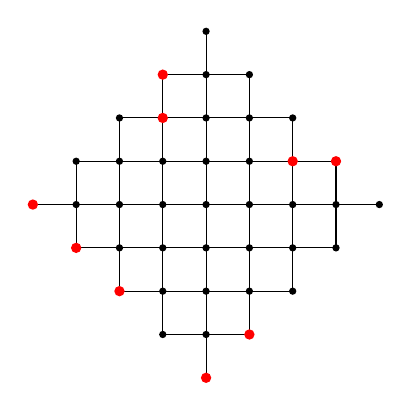
\begin{tikzpicture}[scale=0.55,every node/.style={inner sep=0}]
\draw (4,-4) -- (4,-4);
\draw (3,-3) -- (5,-3);
\draw (2,-2) -- (6,-2);
\draw (1,-1) -- (7,-1);
\draw (0,0) -- (8,0);
\draw (1,1) -- (7,1);
\draw (2,2) -- (6,2);
\draw (3,3) -- (5,3);
\draw (4,4) -- (4,4);
\draw (0,0) -- (0,0);
\draw (1,-1) -- (1,1);
\draw (2,-2) -- (2,2);
\draw (3,-3) -- (3,3);
\draw (4,-4) -- (4,4);
\draw (5,-3) -- (5,3);
\draw (6,-2) -- (6,2);
\draw (7,-1) -- (7,1);
\draw (8,0) -- (8,0);
\fill[black] (4,-4) circle (2.4pt);
\fill[black] (3,-3) circle (2.4pt);
\fill[black] (4,-3) circle (2.4pt);
\fill[black] (5,-3) circle (2.4pt);
\fill[black] (2,-2) circle (2.4pt);
\fill[black] (3,-2) circle (2.4pt);
\fill[black] (4,-2) circle (2.4pt);
\fill[black] (5,-2) circle (2.4pt);
\fill[black] (6,-2) circle (2.4pt);
\fill[black] (1,-1) circle (2.4pt);
\fill[black] (2,-1) circle (2.4pt);
\fill[black] (3,-1) circle (2.4pt);
\fill[black] (4,-1) circle (2.4pt);
\fill[black] (5,-1) circle (2.4pt);
\fill[black] (6,-1) circle (2.4pt);
\fill[black] (7,-1) circle (2.4pt);
\fill[black] (0,0) circle (2.4pt);
\fill[black] (1,0) circle (2.4pt);
\fill[black] (2,0) circle (2.4pt);
\fill[black] (3,0) circle (2.4pt);
\fill[black] (4,0) circle (2.4pt);
\fill[black] (5,0) circle (2.4pt);
\fill[black] (6,0) circle (2.4pt);
\fill[black] (7,0) circle (2.4pt);
\fill[black] (8,0) circle (2.4pt);
\fill[black] (1,1) circle (2.4pt);
\fill[black] (2,1) circle (2.4pt);
\fill[black] (3,1) circle (2.4pt);
\fill[black] (4,1) circle (2.4pt);
\fill[black] (5,1) circle (2.4pt);
\fill[black] (6,1) circle (2.4pt);
\fill[black] (7,1) circle (2.4pt);
\fill[black] (2,2) circle (2.4pt);
\fill[black] (3,2) circle (2.4pt);
\fill[black] (4,2) circle (2.4pt);
\fill[black] (5,2) circle (2.4pt);
\fill[black] (6,2) circle (2.4pt);
\fill[black] (3,3) circle (2.4pt);
\fill[black] (4,3) circle (2.4pt);
\fill[black] (5,3) circle (2.4pt);
\fill[black] (4,4) circle (2.4pt);
\fill[red] (4,-4) circle (3.4pt);
\fill[red] (5,-3) circle (3.4pt);
\fill[red] (2,-2) circle (3.4pt);
\fill[red] (1,-1) circle (3.4pt);
\fill[red] (0,0) circle (3.4pt);
\fill[red] (6,1) circle (3.4pt);
\fill[red] (7,1) circle (3.4pt);
\fill[red] (3,2) circle (3.4pt);
\fill[red] (3,3) circle (3.4pt);
\end{tikzpicture}

\caption{The colour component of the $n=9$ board in diagonal coordinates (case 2: $\DD_{8}$, 41 points), drawn with rook adjacency. Filled points mark one optimal resolving set of size $9$ from Table~\ref{tab:results}; its coordinates are $(0,0),(-1,1),(-2,2),(-4,4),(-3,5),(2,3),(3,3),(1,6),(1,7)$.}
\label{fig:figN9}
\end{figure}

\section{The data}\label{sec:data}

\begin{table}[t]
\centering
\caption{Exact metric dimensions of the two colour components of the bishop's graph $\BB_n$ for $1\le n\le\nmaxverified$ (Theorem~\ref{thm:computed}). The ``conj.''\ columns report whether the exact value equals the conjectured formula of Conjecture~\ref{conj:forms} (checked by the artefact's regression script).}
\label{tab:results}
\small
% AUTO-GENERATED by src/make_paper_assets.py -- do not edit.
\begin{tabular}{rrccccc}
\toprule
 & & \multicolumn{2}{c}{component dimension} & & \multicolumn{2}{c}{matches conj.? \ref{conj:forms}} \\
\cmidrule(lr){3-4}\cmidrule(lr){6-7}
$n$ & $|C_\mathrm{e}|$ & $C_\mathrm{e}$ ($r{+}c$ even) & $C_\mathrm{o}$ ($r{+}c$ odd) & total & $C_\mathrm{e}$ & $C_\mathrm{o}$ \\
\midrule
1 & 1 & 0 & -- & 0 & -- & -- \\
2 & 2 & 1 & 1 & 2 & \checkmark & \checkmark \\
3 & 4 & 2 & 2 & 4 & \checkmark & \checkmark \\
4 & 8 & 3 & 3 & 6 & \checkmark & \checkmark \\
5 & 12 & 5 & 4 & 9 & \checkmark & \checkmark \\
6 & 18 & 5 & 5 & 10 & \checkmark & \checkmark \\
7 & 24 & 7 & 6 & 13 & \checkmark & \checkmark \\
8 & 32 & 8 & 8 & 16 & \checkmark & \checkmark \\
9 & 40 & 9 & 8 & 17 & \checkmark & \checkmark \\
10 & 50 & 10 & 10 & 20 & \checkmark & \checkmark \\
11 & 60 & 12 & 11 & 23 & \checkmark & \checkmark \\
12 & 72 & 12 & 12 & 24 & \checkmark & \checkmark \\
13 & 84 & 14 & 13 & 27 & \checkmark & \checkmark \\
14 & 98 & 15 & 15 & 30 & \checkmark & \checkmark \\
15 & 112 & 16 & 15 & 31 & \checkmark & \checkmark \\
16 & 128 & 17 & 17 & 34 & \checkmark & \checkmark \\
\bottomrule
\end{tabular}


\end{table}

\subsection{Structure of the computed optima}\label{sec:pictures}

The verified optimal sets for $n\le\nmaxverified$ display a stable structure (observations, not theorems):
\begin{itemize}[leftmargin=6mm,itemsep=2pt]
\item by Theorem~\ref{thm:cover}(i), all rows but at most one, and all columns but at most one, carry a landmark; in the computed optima the free row/column is always among the inner lines;
\item in the unshifted cases the extreme corner certificate (Theorem~\ref{thm:cover}(iii)) holds with equality: one of $(0,0)$, $(0,B)$ is always among the landmarks;
\item the excess over the lower bound $\max(W_r-1,W_c-1)$ comes from \emph{cross-pair obstructions}: pairs of cells whose four lines are otherwise landmark-free force dedicated landmarks; the count of forced extra lines grows like one per six lines, the pattern behind the $\floor{W/6}$-type conjectured increments;
\item the reported optima show doubled middle rows/columns (two landmarks in one row/column), consistent with the singleton-cross mechanism of \RRx.
\end{itemize}

\section{Conjecture}\label{sec:conj}

\begin{conjecture}\label{conj:forms}
For all $n\ge2$, let $\dim_1(n)$, $\dim_2(n)$, $\dim_3(n)$ denote the metric dimensions of the diamonds of Theorem~\ref{thm:reform}(1), (2), (3) respectively. Then
\begin{enumerate}[label=\textup{(\roman*)},leftmargin=6mm,itemsep=2pt]
\item $\displaystyle \dim_1(n)=\floor{\tfrac{7n-8}{6}}$ for even $n$;
\item $\displaystyle \dim_2(n)=\floor{\tfrac{7n-5}{6}}$ for odd $n$;
\item $\displaystyle \dim_3(n)=\floor{\tfrac{7n-11}{6}}=\floor{\tfrac{7n-11}{6}}$ for odd $n\ge5$, while $\dim_3(3)=2$.
\end{enumerate}
\end{conjecture}

\begin{corollary}[Asymptotics, conditional]\label{cor:asymp}
If Conjecture~\ref{conj:forms} holds, then in each of the three regimes, with $W$ the diamond row count,
\[
\dim = W+\floor{\frac{W-c}{6}}_+=W+O(1)\quad\text{and}\quad \frac{\dim}{W}\ \longrightarrow\ \frac76 ,
\]
with $c\in\{0,5,4\}$ per case. The dimension exceeds the proved lower bound $\max(W_r-1,W_c-1)$ (Theorem~\ref{thm:cover}) by a $\frac W6$-type offset.
\end{corollary}

The formulas of Conjecture~\ref{conj:forms} match every certified value for $1\le n\le\nmaxverified$ (Table~\ref{tab:results}); they are offered without proof. The $\tfrac16$-per-line increment structure echoes the known exact values for related line-graph families:
\[
\dim\big(K_m\square K_n\big) = \floor{\tfrac{2(m+n-1)}{3}}\quad(m\le n\le 2m-1)\ \cite{caceres2007},
\quad
\dim\big(L(K_n)\big)=\ceil{\tfrac{2n}3}\quad(n\ge6)\ \cite{baileycameron2011},
\]
both of which also sit at $\Theta(W)$ with periodic-type increments, at twice our rate. The unbalanced diamond staircase --- a line graph of an \emph{irregular} bipartite graph, to which the exact theorems of \cite{caceres2007,baileycameron2011} demonstrably do not apply --- apparently obeys a similar law at half the rate; we offer no proof.

\section{Data and code availability}\label{sec:artefacts}

All computations reported here were carried out with the public artefact at
\url{https://github.com/rajveersinh-is-dev/bishops-graph-metric-dimension}:
\texttt{src/bishop.py} (ILP model, HiGHS wrapper, all-pairs BFS), \texttt{src/compute\_dims.py} (direct exact optimisation), \texttt{src/fast\_verify.py} (two-phase certificate ladder), \texttt{src/structure.py} (rule oracle), \texttt{src/conjecture\_check.py} (closed-form regression over all result files), \texttt{tests/} (independent cross-checks), and \texttt{results/} (exact dimensions and full landmark coordinates in JSON). Python 3.14 with numpy/scipy (HiGHS backend) produced all numbers; this document was typeset with Tectonic~0.17. All raw run logs are included with their wall-clock times.

\section*{Declarations}

\emph{Funding:} none.
\emph{Competing interests:} none.
\emph{Data availability:} all data and code are public at the URL above.
\emph{Authorship:} sole author.

\section*{Acknowledgements}
Thanks to the maintainers of HiGHS, \textsf{scipy} and \textsf{Tectonic}.

\bibliographystyle{plain}
\bibliography{references}

\end{document}
